\documentclass[defaultstyle,11pt]{article}

\usepackage{times}
\usepackage[pdftex]{graphicx}
\usepackage{cclicenses}
\usepackage{verbatim}
\usepackage{makeidx}
\usepackage{url} 
\usepackage[hmargin=3cm,vmargin=3.5cm]{geometry}
\usepackage{color}
\usepackage{mathtools}
\usepackage{listings}
\usepackage{hyperref}
\usepackage{amsmath}
\usepackage{nomencl}
\usepackage{multirow}
\usepackage{courier}
\usepackage{caption}
\usepackage{etoolbox}
\usepackage{hyperref}
\usepackage{makeidx}
%\usepackage{xcolor}‎
\makenomenclature

\makeindex

\lstset{
         basicstyle=\footnotesize\ttfamily, % Standardschrift
         %numbers=left,               % Ort der Zeilennummern
         numberstyle=\tiny,          % Stil der Zeilennummern
         %stepnumber=2,               % Abstand zwischen den Zeilennummern
         numbersep=5pt,              % Abstand der Nummern zum Text
         tabsize=2,                  % Groesse von Tabs
         extendedchars=true,         %
         breaklines=true,            % Zeilen werden Umgebrochen
         keywordstyle=\color{red},
    		frame=b,         
 %        keywordstyle=[1]\textbf,    % Stil der Keywords
 %        keywordstyle=[2]\textbf,    %
 %        keywordstyle=[3]\textbf,    %
 %        keywordstyle=[4]\textbf,   \sqrt{\sqrt{}} %
         stringstyle=\color{blue}\ttfamily, % Farbe der String
         showspaces=false,           % Leerzeichen anzeigen ?
         showtabs=false,             % Tabs anzeigen ?
         xleftmargin=17pt,
         framexleftmargin=17pt,
         framexrightmargin=5pt,
         framexbottommargin=4pt,
         %backgroundcolor=\color{lightgray},
         showstringspaces=false      % Leerzeichen in Strings anzeigen ?        
 }
\lstloadlanguages{% Check Dokumentation for further languages ...
         %[Visual]Basic
         %Pascal
         C
         %C++
         %XML
         %HTML
         %Java
}
\DeclareCaptionFont{blue}{\color{blue}} 

\captionsetup[lstlisting]{singlelinecheck=false, labelfont={blue}, textfont={blue}}

\DeclareCaptionFont{white}{\color{white}}
\DeclareCaptionFormat{listing}{\colorbox[cmyk]{0.43, 0.35, 0.35,0.01}{\parbox{\textwidth}{\hspace{15pt}#1#2#3}}}
\captionsetup[lstlisting]{format=listing,labelfont=white,textfont=white, singlelinecheck=false, margin=0pt, font={bf,footnotesize}}

\begin{document}

\renewcommand\floatpagefraction{.9}
\renewcommand\topfraction{.9}
\renewcommand\bottomfraction{.9}
\renewcommand\textfraction{.1}   
\setcounter{totalnumber}{50}
\setcounter{topnumber}{50}
\setcounter{bottomnumber}{50}

\title{GccPy - GCC Front-End for Python}
\author{Philip Herron\\
  \texttt{\url {http://gcc.gnu.org/wiki/PythonFrontEnd}}\\
  \texttt{redbrain@gcc.gnu.org} \\
\byncsa}
\date{\today}
\maketitle
\begin{abstract}
Gccpy is a new front-end to Gnu Compiler Collection which implements the
very popular multi-paridigm dynamic language Python. In here I discuss the
ideas, techniques and aproachs taken to implment this as a staticaly compiled
language.

Ahead of time compiled languages have
been  aimed at 'lower-level' languages such as C/C++/Fortran where the language requires
strong typing and other kinds declarative features; which brings about to some degree much less dynamic
features which languages like Python/PHP/Perl take for granted. More 'high-level' 
languages are able to take advantage of their implementation as interpreted
languages and this allows for this dynamic logic to take place at runtime when a program is passed
through their respective interpreters.

This Paper is licensed under the Creative Commons Attribution Non Commercial Share Alike 2.0 UK: England \& Wales License.
\end{abstract}

\newpage

\tableofcontents
\listoffigures
\lstlistoflistings
\printnomenclature[2.5cm]

\section{Preface}
Gccpy is an attempt at creating a staticly compiled version of Python using GCC as a framework for
middle-end, back-end optimization. Creating statically compiled languages has
been generally aimed for more 'low-level' languages such as C/C++/Fortran where the language requires
strong typing and other kinds declarative features; which brings about to some degree less dynamic
runtime which languages such as Python/PHP/Perl take for granted. These more 'high-level' 
languages are able to take advantage of the fact that they are implemented as interpreted
languages and this allows for much of this dynamic logic to take place at runtime when a program is passed
through their respective implementations.

Here I will explore how Gccpy works and the techniques used to implement this language in such a way,
showing the chalenges faced and solutions proposed.

\subsection{Acknowledgements}
My girl friend Kirsty Johnston for putting up with me late nights, talking about computers; dealing with me in general.
Your an amazing woman!\\
Ian Lance Taylor for all the support he has given me with GCC and making me feel comfortable
with this project. Andi Hellmund who has given so much towards the project in helping flesh out different areas of the compiler.
Linux Outlaws, Jezra, Nybill, Windigo, yaMatt, Fabsh, MethodDan for being great inspiration in the world
of open source and community. Belfast Linux User Group Jonathan McDowel,
Colin Turner, Geoff McCartney, Steve Wilken, comp.compilers, bison and flex community. 
I would like it noted that I was very inspired by for Paul Biggars PhD work into PHC the AOT PHP (PHC) compiler,
to take on this project. WANdisco who don't know but in my spare time I continue to work on this project nearly
like a full time job, Trevor Thompson, Simon Hewitt, Gordon Hamilton, Gavin Shields, Anna Juerk and Trevor Lorimer.

\subsection{Terminology}

\section{Introduction}

The world of programming has been undergoing a paradigm shift in recent years where seemingly very high level
languages like PHP, Python, Java have seen a huge increase in adoption due to the massive resources availble on
regualar computers. With this they are being used for very much more ambitious applications more so each day,
and as such a lot of trust is being put on their respective implementations to provide speed and reliability for
their aplication. All the while providing relativly small development cycles due to the relaxed languages features.

Each language generally has their own niche with, Perl the language of choice for system administration,
PHP for server side scripting, Java-script for client side scripting. Where Python or Ruby could be considered
the new kids on the block with huge communities behind them, and with such large users bases we begin to see
them more and more in everyday applications on the web or our desktops. Perhaps Python on the Linux Desktop
is why python is so popular now rapidly able to use the system and abstract very easily.

Gccpy has been a project to try and implement an ahead of time compiled implementation of Python, to try and
speedup runtime in some areas and create a new style of working with dynamic languages. Most dynamic language implementaions
were and are implemented as interpreters reading in input code and evaluating it statement by statement, where ahead of time
is where we compile the code and link each file together to get a binary removing so much of the front-end parts of an interpreter
and much of the middle end of it to speed up runtime. Though with recent years many projects have begun to implemt their language
using a Jit Just in time compiler to compile just in time to speed up execution Though to understand the idea behind this project
we must first look at all these different styles of implementation which we will cover next.


\section{Approaches and Techniques to Compilation}

I feel its important to draw attention to the different ways of implementing a language and giving an overview of how they work
and why they do so. Before compiling dynamic language as Python, working on a traditional compiler for a strongly-typed language gave much
insight in addressing data and storage. Therefore I want to give an overview of two projects Cmod a compiler for a dialect of
Modula targeted to i386 linux, aswell as an interepter for a basic dynamic language I called crules.

\subsection{CMOD - Modula compiler target to i386 Linux}

This is a traditional compiler where it accepts the input of Modula code and outputs assembler target code for i386 linux. 
This process of producing the output requires alot of optimization and analysis before producing the ouput which I will
show the algorithms and the thought process of doing so.

A compiler consists of three main parts Front-end, Middle-end and Back-end. The Front-end consists of a Lexical
analyser and a parser which generate an \nomenclature{AST}{Abstract Syntax Tree}. This AST is then passed to the
middle-end which over optimizations passes creates the \nomenclature{IL}{Intermediate Language}. In larger
compilers this form can be changed into various optimization forms such as SSA Static Single Assignment form
which makes optimization passes such as constant folding and propagation simpler. But here things are kept simple
and passed onto the back-end to produce the code.

\subsubsection{Typing - Static Weak}
This dialect of Modula much like C has a static typing system but unlike C is not a weak typing system which allows implicit
type conversion which C allows. This makes typing and generating code for this dialect even simpler for us as we dont have to
worry about type conversions and just throw errors if there is.

\subsubsection{Basic Recursive Decent Parser}
The first step of any compiler requires parsing the input before looking at the implemention in Cmod we will look at a basic recursive
decent parser. Parsing code requires a lexical analyser and a parser, the lexical analyser understands regular expressions and returns Tokens
to a parser which evaluates its production rules. An simple example of the language we want to parse is as follows:

\lstset{language=Modula-2,caption={Simple Example},label=Example1}
\begin{lstlisting}
MODULE Example1;
VAR
  X:INTEGER;
BEGIN
  X := 1 + 2 + 3
END Example1.
\end{lstlisting}

The lexer needs to return each token in the input such as the keywords and values we do this by using regular expressions to understand
each token examples would be:

\begin{verbatim}
[0-9]+ DIGIT
\end{verbatim} 
\begin{verbatim}
[_a-zA-Z][a-zA_Z0-9]* IDENTIFIER
\end{verbatim}

Then keywords like MODULE, VAR, BEGIN, a basic overview of an algorithm in C to do this could be:

\lstset{language=C,caption={Simple Lexer},label=Lexer1}
\begin{lstlisting}
enum TOKEN lex_next_token (void)
{
  enum TOKEN retval = EOF;
  for (; *p != '\0'; ++p)
    {
      if (isdigit (*p))
        {
          current_token = atoi (p);
          while (isdigit (*p)) ++p;
          --p;
          retval = DIGIT;
        }
        // handle other items like ';' or ':' the same
      else if (*p == '+') { retval = op_ADD; break; }
        /* we can handle other reserved words in this manner */
      else if (*p == 'M')
        {
          size_t len = 6;
          if (!strncmp (p, "MODULE", len))
            {
              retval = MODULE;
              p += len + 1;
            }
          else
            goto parse_identifier;
          break;
        }
        // .... other reserved words
      else if (isalpha (*p))
        {
parse_identifier:
          current_token = lex_identifier (p);
          /* incr the pointer */
          retval = IDENTIFIER;
          break;
        }
      else if (*p == ' ') continue;
      else break;
    }
    if (retval != EOF) p++;
  return retval;
}
\end{lstlisting}

Now we need to write a parser to use this lexical analyser, but first we need to fomulate a grammar for this language. We can use
\nomenclature{BNF}{Backus Normal Form or Backus–Naur Form} to create a context free grammar definition, which describes the syntax
of the language. BNF is built up of Terminals and Non-terminals, terminal symbols are actual tokens such as DIGIT or VAR, and Non-terminals
are those which build up a symbol based of a sequence of Terminals and non-terminal rules. For example we can have a language that accepts
1,0,1 and the grammar could be as simple as:

\begin{align*}
S &\to \lambda | A , B , A \\
A &\to 1 \\
B &\to 2 \\
\end{align*}

Where S is the start symbol this will only accept the above language, as A resolves to 1 and B resolves to 0 such that we have 101. Then we could
have a language which accepts 10 or 1100 or 111000 and so on, this is an important example as this grammar is reflected in the CMOD compiler.

\begin{align*}
S &\to  L \\
L &\to \lambda | A L B \\
A &\to 1 \\
B &\to 2 \\
\end{align*}

We use a recursive grammar here in that we want 1 and 0 but we can also accept 11110000, which means we work inwards.
L procudes 1 L 0, so if out input is 111000 we have:

\begin{align*}
1 L 0 \\
1 1 L 0 0 \\
1 1 1 0 0 0 \\
\end{align*}

Where each time L resolves to 1 and 0. Creating a basic parser you can follow this style of algorithm:

\lstset{language=C,caption={Simple Parser},label=Parser1}
\begin{lstlisting}
int parse_accept (enum TOKEN ac)
{
  if (t == ac)
    {
      t = lex_next_token ();
      return 1;
    }
  else
    return 0;
}

int parse_expect (enum TOKEN ac)
{
  if (parse_accept (ac))
    return 1;
  printf ("unexpected symbol!\n");
  parse_err = true;
  return 0;
}
\end{lstlisting}

And you can use a series of parser accept or expect to parse out declarations, this forms a basic parser. When
implementing the Compiler the toplevel general algorithm to follow is:

\lstset{language=C,caption={Driver},label=Driver}
\begin{lstlisting}
int cm_do_compile (const char * in)
{
  /* call parser which fills up the translation unit for us... */
  retval = cm_parse_file (in);
  ERROR_CHECK;

  /* Do checks and some transformations on the IR */
  cm_dot_check_translation_unit (translation_unit);
  ERROR_CHECK;

  cm_target_gen_ASM__ (translation_unit,t_out,in);

  return retval;
}
\end{lstlisting}

This is the main driving code in a compiler calling parse is the front-end and check is the middle-end optimizer and gen-asm
is the back-end. We will up the translation unit with our declarations from the parser and keep optimizing as we go.

\subsubsection{Front-End - Parsing}
In Cmod I use Flex which is a lexical analyser generator and Bison a LALR parser generator. We input a series of definitions
for both and we get a parser which is very well suited a compiler and is very easy to maintain. The lexer which is generated
works very similar to our example and follows the same kind of algorithm and idea. An LALR parser uses Stacks and States
pushing tokens onto a stack and moving into new states and resolving and pop'ing tokens off the stack in each action illustrated
in figure \ref{fig:LR parser}.

\begin{figure}[h!]
  \caption{LR parser}
  \label{fig:LR parser}
  \centering
    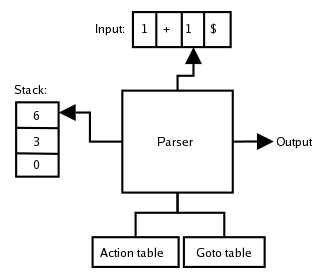
\includegraphics[width=0.5\textwidth]{LR_Parser.png}
\end{figure}

As we walk though the input from listing \ref{Example1} we create our AST and create binary's also known
as Acyclic Graphs like in figure \ref{fig:DAG}.

\begin{figure}[h!]
\centering
 \label{fig:DAG}
 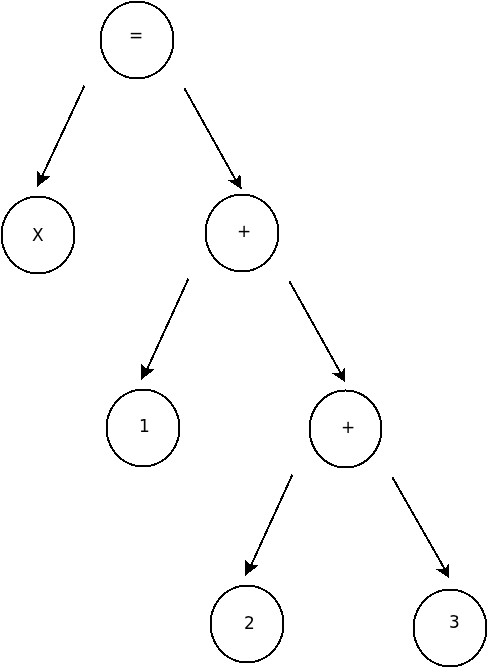
\includegraphics[totalheight=0.3\textheight, width=0.3\textwidth]{DAG1.png}
\end{figure}

These are represented by using these types of functions \ref{TreeApi}.

\lstset{language=C,caption={Tree API},label=TreeApi}
\begin{lstlisting}
build_decl (VAR_DECL, type, id, NULL_TREE);
build_decl (MODIFY_EXPR, NULL_TREE, opa, opb);
build_decl (ADD_EXPR, NULL_TREE, opa, opb);
\end{lstlisting}

At this stage our parser will produce this code:

\lstset{language=C,caption={Example1 - IL - 1},label=Example1-IL-1}
\begin{lstlisting}
void Example1 ( void )
{
	int X; 

	X = 1 + 2 + 3;
}
\end{lstlisting}

This is our AST form which we can pass to the middle-end for optimization before passing to the middle-end.

\subsubsection{Middle-end - Static Analysis}
This form isn't ready for back-end code generation, we must first lower this a little further to make things simpler to process.
Everything can be broken down to 3 items, an operation with operands A and B; this makes code generation
much simpler since instruction sets generally consist of an instruction and operands.
This can sometimes be referred to as a 3 address code, its similar to a static single assignment
form SSA, which is used to make compiler optimizations simpler, but we don't do this here but there is room in the compiler
for optimization passes which I will disccuss later.

Evaluation of expressions such as the listing \ref{Example1-IL-1} requires us to break down its Tree form shown in \ref{fig:DAG}. As
each root of each contains an operation with 2 operands we can quite easily form an intermedite form shown in listing \ref{Example1-IL-2}

\lstset{language=C,caption={Example1 - IL - 2},label=Example1-IL-2}
\begin{lstlisting}
T.0 = 1 + 2;
T.1 = T.0 + 3;
X = T.1;
\end{lstlisting}

To achieve this we recursivly walk down the tree in src/ii-mod-dot.c you can follow the function (void cm\_dot\_check\_expression (tree ** decl)).
The general algorithm is:

\lstset{language=C,caption={Expression Evaluation 1},label=ExprEval1}
\begin{lstlisting}
void walk_expr (tree decl)
{
  switch (TREE_CODE (decl))
    {
      case IDENTIFIER:
        retval = lookup_var_decl (decl)
        break;

      case SCALAR:
        retval = decl;
        break;
        ...
      default:
        {
          switch (TREE_CODE (decl))
            {
              case MODIFY_EXPR: fold_modify (decl) break;
              default: fold_bin_expr (decl) break;
            }
        }
      break;
    }
}
\end{lstlisting}

Variable lookup in the middle-end is handled by a stack of hash-tables, where by for each declaration in the modula language it
requires declaration of variables. So we fill this up at the begining with these VAR\_DECL nodes. So when we come across an identifier
node we simply hash the string and lookup the stack of tables for the VAR\_DECL if we find it all is good we found the reference we were
looking for. Otherwise we throw and error in fold\_modify and return an error\_mark\_node meaning it was an undeclared variable.

When we fold binary expressions such as addition the algorithm we use would look like:

\lstset{language=C,caption={Expression Evaluation 2},label=ExprEval2}
\begin{lstlisting}
cm_vector_t * fold_bin_expr (tree decl)
{
  cm_vector_t * t1 = NULL, * t2 = NULL;

  tree op = NULL;
  tree opa, opb, t1op, t2op, tmp_var;

  opa = TREE_LHS (decl);
  opb = TREE_LHS (decl);

  t1 = walk_tree (opa);
  t2 = walk_tree (opb);
  
  t1op = cm_vec_pop (t1);
  t2op = cm_vec_pop (t2);
  tmp_var = create_new_tmp_var (TREE_TYPE (decl));

  tree *o = build_decl (TREE_CODE (decl), TREE_TYPE (decl),
                        t1op, t2op);
  op = build_decl (MODIFY_EXPR, TREE_TYPE (decl), tmp_var, o);

  cm_vec_push (t1, op);
  cm_vec_push (t1, tmp_var);

  return t1;
}
\end{lstlisting}

This kind of function will walk down the left and right side of a tree and return a vector of operations with a tmp
variable storing the folded expression result which you can use to access the result of an operation. So if 1 + 1 was
the input we would get a T.0 = 1 + 1 and T.0 on the stack. And the walk\_tree would fold out the scalars and any other
references, or even other expression. So if we take our original input \ref{Example1} we would produce \ref{Example1-IL-3}.

\lstset{language=C,caption={Example1 - IL - 3},label=Example1-IL-3}
\begin{lstlisting}
void Example1 ( void )
{
	int X; 
	int T.0; 
	int T.1; 

	T.0 = 1 + 2;
	T.1 = T.0 + 3;
	X = T.1;
}
\end{lstlisting}

Its important to note any tmp variables are automatically added to the chain of VAR\_DECL node's per block declaration. This
is important for the back-end to allocate enough space for the operations to run correctly. Now that we see how basic expressions
can be handled we need to look at other examples like control structures, calls and contigious data structures like arrays. For a
control structure we will look at conditionals and example of which is \ref{condit}.

\lstset{language=Modula-2,caption={Example2 - Conditionals},label=condit}
\begin{lstlisting}
MODULE Example2;

VAR
  X:INTEGER;

BEGIN
  X := 1 + 2 + 3;
  IF X<5 THEN
     X := X + 1
  END
END Example2.
\end{lstlisting}

We read this in and need to fold out to this, we create a basic jump table system where by the if
operation is simply if T.2 is greater than 0 it evalues true, if it is 0 or less it evaluates false
and we goto where nesecary.

\lstset{language=C,caption={Example2 - Conditionals- IL},label=condit-fold}
\begin{lstlisting}
void Program4 ( void )
{
	int X; 
	int T.0; 
	int T.1; 
	int T.2; 
	int T.3; 

	T.0 = 1 + 2;
	T.1 = T.0 + 3;
	X = T.1;
	T.2 = X < 5;
	if (T.2)
	  {
		goto .C.0;
	  }
	else 
	  {
		goto .C.1;
	  }
	
.C.0:
	T.3 = X + 1;
	X = T.3;
	goto .C.1;
	
.C.1:
}
\end{lstlisting}

Loops can be handled in a similar manar tranform something like \ref{Loops}:

\lstset{language=C,caption={Loops},label=Loops}
\begin{lstlisting}
for ( i=0; i<10; ++i ) { do_some stuff }
into 3-address code instructions using a label something like:
                      - I := 0;         ;; the initilizer
                      - goto label_for_loop__checks;
 * label_for_loop__start:
                      - do_some_stuff
                      - I := I + 1;     ;; the incrementor
 * label_for_loop__checks:
                      - if (i<10) { goto label_for_loop__start; }  ;; the loop_conditional
                      - { continue on with rest of program }
\end{lstlisting}

So really any control structure can be handled by jump tables. Now that the middle-end has
optimized the IL we have a very linear and simple program to generate code for.

\subsubsection{Back-end - Code-generation}

Code generation I approached from first-principles and used states to manage
my cpu\_state which represented the 4 main general purpose registers on an i386 machine.
The translation unit of tree declarations is a vector of function declarations of all the
same signiture of void identifier (void), which keeps things simple. When we walk into a
function decl we must first walk its VAR\_DECL node and figure out how much space we need to
allocate for the locals.

\subsection{Crules - Interpreter}

\subsection{Virtual Machines - overview}

\subsubsection{Just-in-time compilation}
\nomenclature{jit}{Just-in-time compilation}

\section{Python and Gccpy}

To compile python first implementing dynamic typing had to be the focus, since everything
within the language revolves around the concept of any name being able to store data of seemingly
any size. For example python will allow expressions such as \ref{Dynamic1}.

\lstset{language=Python,caption={Dynamic Typing 1},label=Dynamic1}
\begin{lstlisting}
x = 1
x = 1.5
x = 'c'
x = "string"
x = [ 1, 2, 3, 4 ]
x = [ 1, "string", 'c', 1.5 ]
x = [ 1, "string", 'c', 1.5, [ 1, 2, 3 ] ]
\end{lstlisting}

The way this style of dynamic typing was implemted is by treating a name such as 'x' is simply pointing to
data; rather than in languages such as C where names store data.

The next to think of was how names and attributes can be accessed aswell how names within the running of the program
are addressed to preserve consistancy. Other main pitfalls inculde how calls are handled which had to be at runtime
due to being unable to fully known which method or call your wanting to call simply from the name example \ref{ambig}:
if you consider both of those foobar declarations in seperate programs. How you call the class or the method are completely
different though when we see the call to foobar it simply looks the same.

\lstset{language=Python,caption={Ambigious calls or names},label=ambig}
\begin{lstlisting}
class foobar:
    def __init__ (self):
      pass

def foobar():
  dosomething ()

foobar ()
\end{lstlisting}

Its quite simple how we handle this in that we lookup the name foobar and call the call hook on the object and thusly
on a per object type basis in this case static method vs Class object. Each of their respective implementations understands
how to handle this. Then how are expressions handled we simply can have a binary operator table on a per object basis defining
how these are handled.

\subsection{Getting gccpy and usage}

There are no official releases of gccpy yet as much of it is still under heavy development. But you can access stable'ish code
from \ref{install}. Then you can view more development code at \url{http://code.redbrain.co.uk/cgit.cgi/gccpy/}.

\lstset{language=Bash,caption={Installing Gccpy},label=install}
\begin{lstlisting}
# git clone git://gcc.gnu.org/git/gcc.git
# git checkout --track -b origin/gccpy gccpy
# mkdir gccpy-build
# cd gccpy-build
# ../gccpy/configure --enable-languages=python --disable-bootstrap
# make
# make install
\end{lstlisting}

This will install 3 things gccpy and gpy1, which are the compiler driver and compiler proper respectivly and also libgpython.so
which is the runtime library.

\subsection{Compilation pipeline}
Gccpy is quite a complicated compiler, it isn't simply a front-end to gcc in the traditional sense, such that we simply parse code
into GENERIC and let GCC handle the rest for us. The first hurdle was parsing python into an un-typed IR which I designed called DOT.
This is a similar design pattern to gccgo for golang which Ian Taylor created for Google. Though gccpy requires several more steps of
optimization before we can compile python. Gccpy has its own pass manager and we have several passes of optimization then the final
two passes to pass the generated code to the GCC middle-end.

\begin{itemize}
  \item py-dot-pass-check1.c
  \item py-dot-pass-const-fold.c
  \item py-dot-pass-translate.c
  \item py-dot-pass-pretty\_print.c
  \item py-dot-pass-types.c
  \item py-dot-pass-genericify.c
\end{itemize}

Each of these passes are called in this order and I will show in detail what and why each of these exist. The first things
within the front-end we parse the code using Flex and Bison and then we are in the pass system with the DOT IL.

\subsection{Parsing Python}
Parsing python was a real challenge in that python has requirements on whitespace for indentation, which is tricly to handle.

\subsection{DOT untyped Intermedite Language}
DOT.

\subsection{Sanity Checks - py-dot-pass-check1.c}

\subsection{Constant Folding/Propagation - py-dot-pass-const-fold.c}

\subsection{Translation - py-dot-pass-translate.c}

\subsection{Pretty Printer - py-dot-pass-pretty\_print.c}

\subsection{Type Generation - py-dot-pass-types.c}

When we enter this pass our goal is to generate the types from the python code so for example we take \ref{types1} and generate \ref{types2}.

\lstset{language=Python,caption={Types Example 1},label=types1}
\begin{lstlisting}
class foobar:
  x = 1
  y = 2
  def __init__ (self):
    self.z = x

x = 1
x = foobar ()
x = x.y
\end{lstlisting}

\lstset{language=Python,caption={Types Example 2},label=types2}
\begin{lstlisting}
struct foobar {
  gpy\_object\_t *x, *y, *z,
  *__init__, *__field_init__;
};

struct main_module {
  gpy_object_t * x, *foobar;
};
\end{lstlisting}

To generate these types we must remember things such that class attributes dont need to be declared before they are intilized.
If you look at \ref{types1} the class intilizer has self.z being assigned

\subsection{Genericification - py-dot-pass-genericify.c}

\subsubsection{Runtime - libgpython.so}

\subsubsection{Compilation vs Runtime}
Overall I want to draw attention to thought this project the whole dynamic of finding compilation vs runtime has been the
main problem. Its very easy to want to write alot of code to evaluate things in the runtime library and much of it is unavoidable
though at compile time is where we want to keep things.

% =======================================================

\newpage

\section{References}

\subsection{Links}

\subsection{Index}
\printindex

\bibliographystyle{plain}
\begin{thebibliography}{9}

	\bibitem{lolcode}
	  Lolcode Team,
	  http://lolcode.com/

\end{thebibliography}

\end{document}
